%! Author = Philipp Emmenegger
%! Date = 30/06/2021

\section{Authentication}
\textbf{Confidentiality:} Protects transmitted data against eavesdropper.\\
\textbf{Integrity:} Provides protection against modification.\\
\textbf{Availability:} Data needs to be available when needed.\\
\textbf{Non-repudiation:} No one can deny an action.\\
\textbf{Identification:} Username connects to a person.\\
\textbf{Authentication:} Verifying a claim of identity with:
\begin{itemize}
    \item Something you know
    \item Something you have
    \item Something you are
\end{itemize}
\textbf{Authorization:} Determines what resources a user can access.\\

\subsection{Software Token}
\textbf{TOTP:} Time-based One-time Password
\begin{itemize}
    \item Often used as 2nd factor
    \item Based on keyed-hash message authentication code
\end{itemize}

\subsection{Basic Auth}
\begin{itemize}
    \item Load balancer
    \item Services (keep state!)
    \item Only with HTTPS
    \item Can be encoded in URL: \textit{user:pw@domain}
    \item Server will reply with header: \textit{WWW-Authenticate}
\end{itemize}

\subsection{Digest Auth}
\begin{itemize}
    \item Based on Basic Auth
    \item Also available in traefik
    \item Hash + nonce, against replay attacks
\end{itemize}
\textbf{Advantages}
\begin{itemize}
    \item PW not in clear text (MD5), can be SHA-256
    \item Nonce for replay protection for client/server
\end{itemize}
\textbf{Disadvantages}
\begin{itemize}
    \item Browser L\&F
    \item Cannot use scrypt or bcrypt to store PWs
\end{itemize}

\subsection{Create SSL CA certificates for server}
\begin{itemize}
    \item Create CA
    \item Create certificate
    \item Add nginx security in your local network
\end{itemize}

\subsection{Session-based authentication}
\begin{itemize}
    \item Sticky session required
    \item Authenticate in Service Instance
\end{itemize}

\subsection{JWT}
\begin{itemize}
    \item Stateless
    \item All server instances know a secret token / public key
    \item When user logs in, server send back token
    \item Client sends: Authorization: Bearer <token>
    \item Client can store token in local storage
\end{itemize}

\subsubsection{Access Token / Refresh Token}
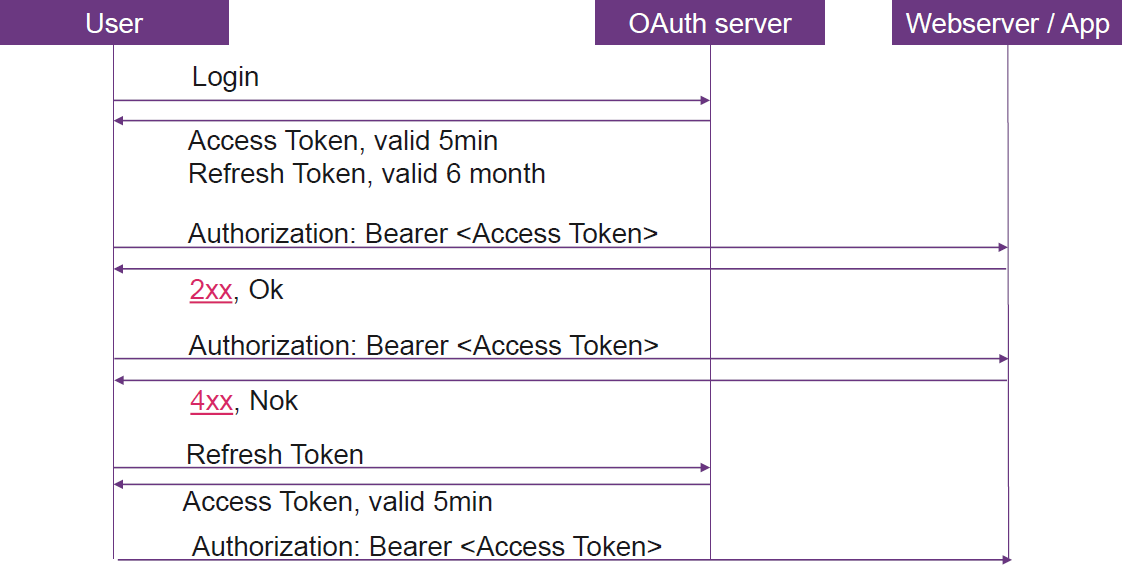
\includegraphics[width=\linewidth]{img/jwt.png}
\textbf{Access Token}
\begin{itemize}
    \item Short lifetime (10min)
\end{itemize}
\textbf{Refresh Token}
\begin{itemize}
    \item Used to get a new access token
    \item IAM / Auth server creates access tokens
\end{itemize}
